\chapter{Methods}
\label{chap:methods}

The methods presented in this thesis were drawn from a desire to exploit information from a local neighborhood around a residue when performing interface prediction.
The biological motivation is that a residue's neighborhood influences its propensity to participate in an interface.
It was noted in Chapter \ref{chap:neuralnetworks} that convolutional neural networks are one way of detecting features in a local neighborhood, but are limited to regular grids. 
Unfortunately, proteins cannot naturally be represented as a regular grid, so convolutions must be developed for a more natural representation, graphs.


\section{Proteins As Graphs}

An undirected, unweighted graph $G$ consists of a set of vertices, $V=\{v_1, v_2, ..., v_n\}$, and a set of eges, $E=\{e_1, e_2, ..., e_m\}$ where each edge is incident to two vertices and there is at most one edge between two vertices.
In a protein graph, each vertex represents a residue in the protein, and each edge represents the relationship between two residues.
Thus any information pertaining to a particular residue can be associated with the relevant vertex in the form of a feature vector.
The features used in this work are drawn from features used in prior interface prediction work \cite{minhas2014} and pertain to the sequence conservation and the structure of a particular residue. 
Likewise, any information pertaining to the relationship between two residues can be associated with the relevant edge.
The edge features used here describe the distance between and relative orientation of two residues.
These edge features are defined between any two residues in the protein, so the graph is complete. 
The number of edge features and number of vertex features may not be the same.
A detailed explanation of each feature is contained in Appendix \ref{appendix:features}

This representation is a structural abstraction of the original protein to a well studied mathematical object.
It does not rely on a coordinate system, as is the case when working with raw 3D positions.
This makes biological sense because proteins often have no natural orientation in the cell, and the relative orientations of two interacting proteins is not known a priori.
However, the graph retains 3D structural information in the edge features, and is embedded in an underlying metric space.
This property is useful when defining local neighborhoods around vertices, which is necessary when designing convolutions.
With proteins represented as graphs, the remaining task is to design a convolution operation which operates on graphs. 

\section{Graph Convolutions}
Though the formulation and application of graph convolutions presented in this thesis are new, graph convolutions have existed in the literature for several years.


\subsection{Prior Work In Graph Convolutions}
Recent years have seen increased attention for problems involving graph structured data, prompting developments in graph convolutions to perform various tasks on those data~\cite{bronstein2016}.
These approaches have generally fallen into two categories, \textit{spectral} and \textit{spatial}.

Spectral methods are based on linear functions in the "frequency domain" of a graph, defined using the laplacian operator $\mathcal{L}=I-D^{-1/2}WD^{-1/2}$, where $W$ is a similarity matrix (containing edge weights), and $D$ is a diagonal matrix containing the degree of each vertex~\cite{bruna2013}\cite{henaff2015}\cite{kipf2016}.
%TODO: mention(?): scaling to large graphs difficult because factoring large matrices difficult
Each filter in a spectral convolution implies a weighting of each frequency in the spectral decomposition of the graph~\cite{mallat2009}.

Spatial methods instead define operations in a localized neighborhood of a vertex~\cite{henaff2015}\cite{atwood2016diffusion}.
Each neighborhood constitutes a receptive field where a convolution operation is performed. 
Convolutions commonly involve a vector of weights and take a weighted sum of neighbors, much like a discrete convolution on a grid can be viewed as taking a weighted sum of grid elements within the receptive field.
%TODO: cite papers with different neighborhood convolutions (write more about them?)
Spatial convolutions are more directly analogous to grid based convolutions as described in Chapter \ref{chap:neuralnetworks}, but introduce a problem of correspondence when translated to graphs.

\subsection{The Problem of Receptive Field Correspondence}
When convolving on a grid, each receptive field has an identical structure (for example 3x3 pixels in an image), so there is an automatic correspondence between receptive fields, such  that the same weights are applied to corresponding portions of all receptive fields. 
For example, the upper left pixel in a 3x3 receptive field is always multiplied by the same weight when taking the weighted sum, regardless of which receptive field is being considered.
With graphs, there is often no such correspondence from one receptive field to another (there is no "upper left" vertex in a vertex neighborhood), in fact, the number of neighbors in a receptive field may not be constant and is dependent on how the receptive field is defined.
This problem of correspondence has been addressed in various ways in the literature and are summarized below. 
\begin{enumerate}
	\item \textit{Imposed ordering of neighbors}. This approach generates a correspondence between two receptive fields by ordering the neighbors in each and associating neighbors of a common position. 
	Ordering methods can be based on vertex characteristics like degree and betweenness centrality, or some domain specific knowledge ~\cite{niepert2016}\cite{duvenaud2015}.
	They also typically require the number of neighbors in a receptive field to remain the same.
	This approach allows filter weights which are coupled to a particular position in the ordering, which hopefully has some invariant significance across all receptive fields.
	
	\item \textit{Identical treatment of neighbors}. This approach ignores the need to establish a correspondence between receptive fields and instead treats all neighbors in the same way.
	Rather than applying different weights to neighbors depending on their position in an ordering, the same weights are applied to each neighbor.
	This allows for different sizes of receptive fields and avoids choosing an ordering method, but lacks the ability to treat neighbors differently based on their relationships to each other and to the central vertex.
\end{enumerate}
Figure \ref{fig:correspondence_approaches} shows a graphical depiction of both approaches.

\begin{figure}
	\centering
	%\begin{center}
	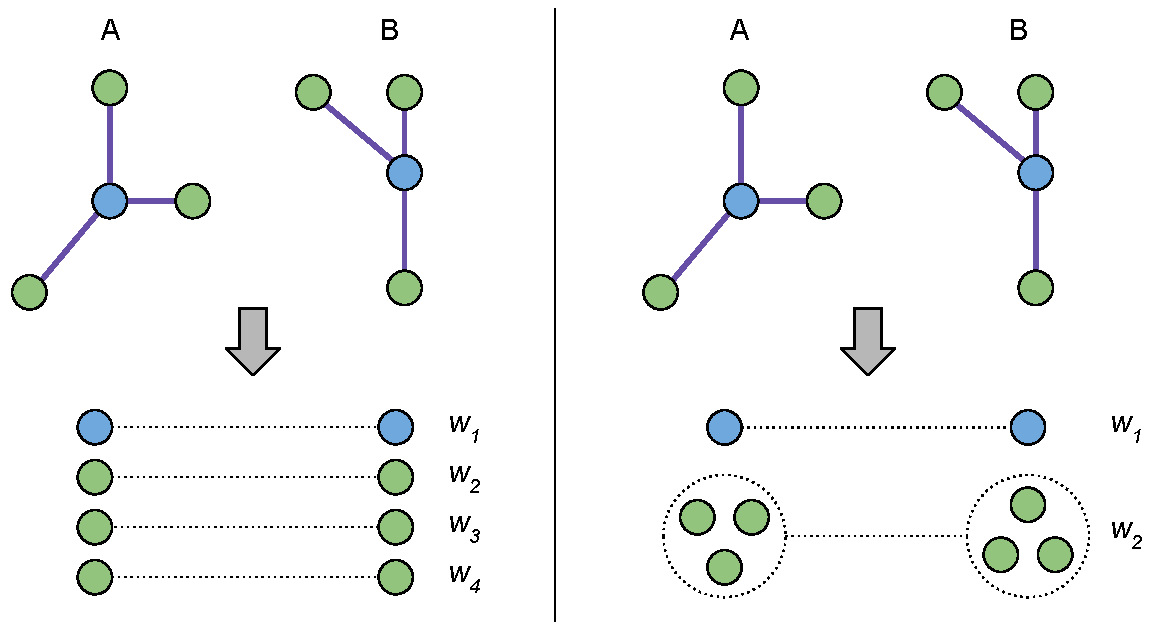
\includegraphics[width=0.8\textwidth]{correspondence_approaches.pdf}
	%\end{center}
	\caption{Two approaches of establishing correspondence between the neighbors of receptive fields A and B. Central vertices are shown in blue and neighbors in green. The central vertices always correspond with one another. Left: neighbors are ordered and associated based on position. Unique weights (\textit{$w_2$--$w_4$}) can then be applied to each position in the order. Right: neighbors are left unordered and treated identically. This requires that the same weights (\textit{$w_2$}) be used for all neighbors.}
	\label{fig:correspondence_approaches}
\end{figure}


\subsection{Order Free Coupled Graph Convolutions}
This thesis presents a structural convolution which avoids imposing an arbitrary ordering on the neighbors in a receptive field but also avoids treating all neighbors the same.
This is accomplished by incorporating information from the edges between each neighbor and the central vertex.
There are two variants of graph convolution which differ in how the edge information is incorporated, denoted \textit{sum coupled} and \textit{product coupled} respectively.
For a central vertex $i$ on the graph and a local neighborhood of vertices $\mathcal{N}_i$, the output of a sum coupled graph convolution is:
\begin{equation}
h_i(x | W^\textsc{c}, W^\textsc{n}, W^\textsc{e}, b) = \sigma \bigg( W^{\textsc{c}} x_i + \frac{1}{|\mathcal{N}_i|}\sum_{j \in \mathcal{N}_i} W^{\textsc{n}} x_j + \frac{1}{|\mathcal{N}_i|}\sum_{j \in \mathcal{N}_i} W^{\textsc{e}} A_{ij} + b \bigg),
\label{eq:sum_coupling}
\end{equation}
where $x_i$ is the feature vector associated with vertex $i$, $A_{ij}$ is the feature vector associated with edge $(i, j)$, $W^\textsc{c}$, $W^\textsc{n}$ and $W^\textsc{e}$ are weight matrices, and $b$ is a vector of biases. 
If there are $L$ vertex channels, $P$ edge channels, and $K$ filters, then $W^\textsc{c}\in\mathbb{R}^{KxL}$, $W^\textsc{n}\in\mathbb{R}^{KxL}$, $W^\textsc{e}\in\mathbb{R}^{KxP}$, and $b\in\mathbb{R}^{K}$.
Intuitively, this calculates an activation for the central vertex, each neighbor vertex, and each edge between a neighbor and the central vertex separately
Even though the same weight matrix is being applied to every neighbor, this incorporate information about how each neighbor relates to the central vertex, allowing differentiation between neighbors.

This formulation loses the association between a neighbor and the edge which connects it to the central vertex. 
Therefore an alternative formulation, product coupled graph convolution, is defined as:
\begin{equation}
z_i = \sigma \bigg( W^{\textsc{c}} x_i + \frac{1}{|\mathcal{N}_i|}\sum_{j \in \mathcal{N}_i} (W^{\textsc{n}} x_j) \odot (W^{\textsc{e}} A_{ij}) + b \bigg),
\label{eq:prod_coupling}
\end{equation}
where $\odot$ denotes the elementwise product between two vectors or matrices. 
In this formulation, each vertex signal is multiplied by the signal of the edge which connects it to the central vertex.
This allows a neighbor's influence on the overall activation to be modulated by its relationship to the central vertex.
For protein graphs, this means neighboring residues will contribute more or less to the activation depending on their distance from and relative orientation to the central vertex, with the precise modulation determined by the edge activations.

Both sum coupled and product coupled graph convolutions are invariant to rotations or translations in space, don't impose an ordering in the neighbors or a correspondence between receptive fields of any kind, allow for different numbers of neighbors, and account for the different relationships between neighbors and the central vertex. 
The receptive fields are always defined around a central vertex, so the results of convolution can be applied to that vertex.
This retains the graph structure after each convolution, so convolutional layers are stackable, as with images.

A note on receptive fields: 
the graphs used in this thesis are complete and embedded in a metric space, so a receptive field can be defined using a threshold $\delta>0$ such that all vertices closer to the center vertex than the threshold are included in the receptive field.
All neighbors in a receptive field are guaranteed to share an edge with the central vertex, allowing the application of equations \ref{eq:sum_coupling} and \ref{eq:prod_coupling}.
For incomplete graphs, a receptive field can be defined as all vertices within $k$ hops of the central vertex. 
If $k=1$, both versions of graph convolution can directly be applied.
If $k>1$, then product coupled graph convolution can't be directly applied to neighbors more than 1 hop away from the center vertex, since they share no edge with the center. 
Though there are ways to adapt product coupled graph convolution in this situation, they are not the focus of this thesis.
%TODO: say more?

These graph convolutions allow the detection of local patterns on a single graph, and produce a new representation at each vertex.
Partner specific protein interaction, however, requires classifying pairs of residues in different proteins (vertices in different graphs), which is essentially making predictions in the product graph. Such predictions are made using a pairwise neural network architecture.

\section{Pairwise Deep Learning Architecture}
A pairwise architecture is comprised of three main sections: the \textit{pre-merge} (or \textit{leg}) layers, the \textit{merge} layer, and the \textit{post-merge} layers.
See Figure \ref{fig:pairwise_arch1} for a graphical depiction.
Even though predictions are being made for pairs of individual residues, convolution depends on surrounding residues, or in the case of stacked convolutional layers, the generated representation of surrounding residues.
Therefore it is less redundant to convolve an entire protein at once than create (and recreate) convolutional representations for a vertex whenever it is involved in a pair or the receptive field of a vertex in a pair.
Therefore the input to a pairwise classifier neural network is a pair of protein graphs derived from the \textit{ligand} and \textit{receptor} in a known protein complex.
Each protein is convolved individually in a separate leg, where the number of convolutional layers in each leg is the same and model weights and other parameters are shared across the legs.

The merge layer then combines the vertex representations from one graph with the vertex representations from the other into pairs. 
In theory, this merge process should be symmetric because the network should perform identically regardless of which protein is used as input into which leg.
For example, the elementwise sum, elementwise product, and outer-product are all commutative and therefore produce symmetric output.
Another option is to combine pairs asymmetrically, such as concatenating the two representations together, but then average the predictions between each ordering of the representations.
This also ensures symmetric network behavior.
%TODO: talk about pairwise kernels?

After merging, the resultant combined representation for each pair of residues is passed through a number of post-merge layers until reaching the last layer, which has a single output for each pair indicating the prediction for that pair
This output is be compared to an encoded label indicating whether or not the pair constitute part of the true interface. 

\begin{figure}
	\centering
	%\begin{center}
	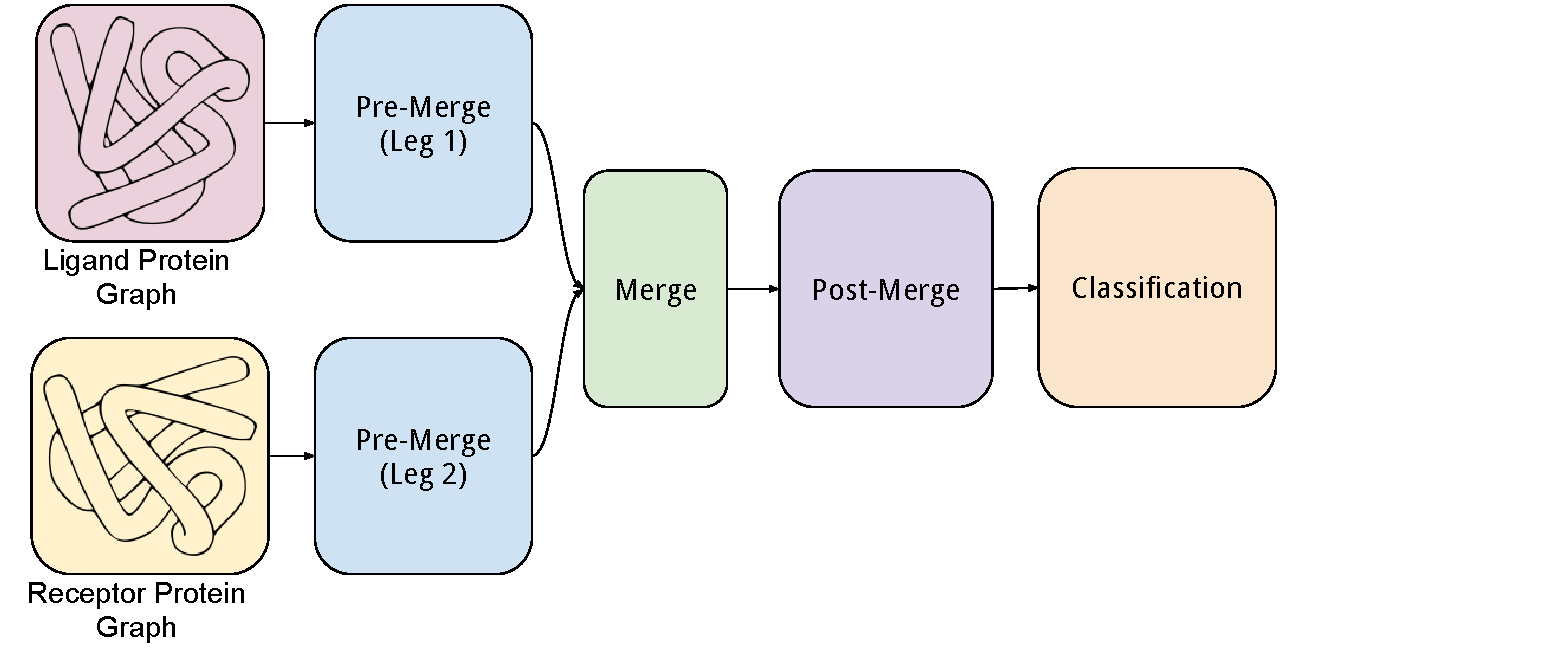
\includegraphics[width=0.8\textwidth]{pairwise_network1.pdf}
	%\end{center}
	\caption{.}
	\label{fig:pairwise_arch1}
\end{figure}

This chapter has laid out the major components necessary to perform graph convolutions
